\section{Literature Review}\label{chap:review}
The close-contact sublimation models presented in this thesis build upon established research, the most important being the theory of close-contact melting. Before we delve into a review of the most important theoretical concepts, we aim to familiarize the reader with the contents of this thesis in the context of existing literature. 



\begin{figure}[ht!]
\centering
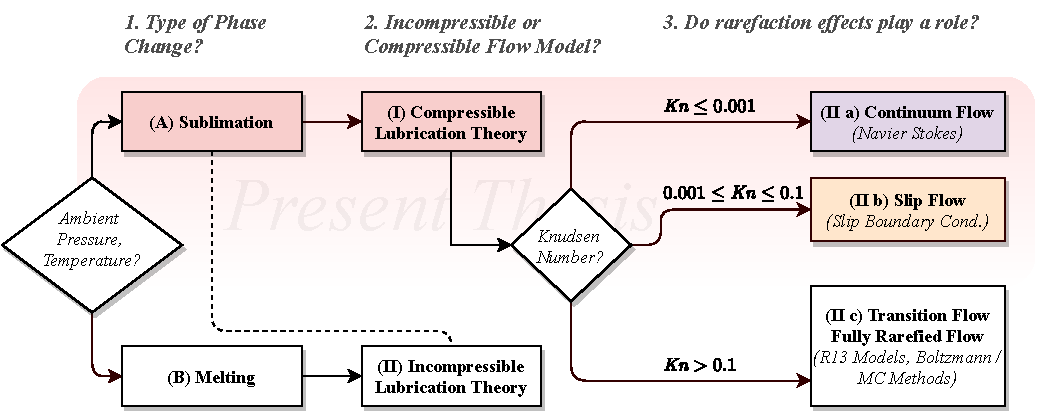
\includegraphics[trim=0 0 0 0 cm,clip,width=1\textwidth]{Chapters/Review/figs/workflowhorizontal/ccmworkflowHorizontal.pdf}
\caption[Close-Contact Phase Change: Case Distinction Based on Physical Regimes]{Case distinctions for different physical settings. We consider the phase transitions from a solid (icy) state to either  gaseous \textbf{(A)} or liquid \textbf{(B)} state. In this thesis, we study close-contact sublimation \textbf{(A)}. In particular, we investigate compressibility effects \textbf{(I)} in the gas film. The shading indicates the main subjects covered in this thesis. \textit{A hybrid regime of partial sublimation and partial melting is not discussed in this thesis and thus excluded from the sketch.}}
\label{fig:ccmcworkflow}
\end{figure}

Figure \ref{fig:ccmcworkflow} sketches modeling approaches to close-contact phase change in different flow regimes. Depending on the ambient conditions, we consider solid-gas sublimation (\textbf{A}) or solid-liquid melting (\textbf{B}).
The present thesis aims to expand the existing close-contact melting theory for incompressible melts by adding a model for solid-gas sublimation phase change (\textit{shaded boxes, top half} of Fig. \ref{fig:ccmcworkflow}). 
White boxes contain topics that are either established in literature and reviewed in the following sections (\textbf{B}, \textbf{II}) or not covered in this thesis (\textbf{II c}). \textit{In the following paragraphs, bold labels refer to Fig. \ref{fig:ccmcworkflow}, if not stated otherwise.}

To make the discussion of close-contact phase change in the context of melting probes more accessible, we discuss a short conceptual sketch (Fig. \ref{fig:introEquilibria}) of a simple rectangular melting head at constant temperature $T_H$, moving through solid ice at a constant velocity $U$.

\begin{figure}[ht!]
\centering
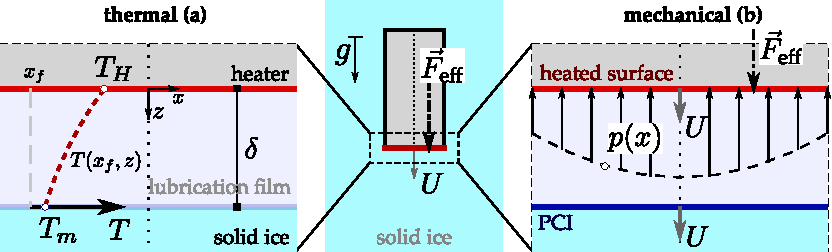
\includegraphics[trim=0 0 0 0 cm,clip,width=1\textwidth]{Chapters/Review/figs/equilibriaIntro/equilibriaSketch.pdf}
\caption[Equilibrium in Close-Contact Phase Change]{Close-contact equilibrium state in the lubrication film at the tip of a flat constant temperature melting head sinking through an icy environment with velocity $U$. The zoomed in views of the melt (\textit{film thickness} $\delta$ \textit{not to scale}) show an example temperature distribution $T(x_f,z)$ at some arbitrary fixed location $x_f$ (\textbf{a}) and the mechanical equilibrium between the pressure $p(x)$ in the lid and the effective external force $F\ts{eff}$ (\textbf{b}).}
\label{fig:introEquilibria}
\end{figure}

The probe's heated surface induces a phase change from solid to liquid (\textit{close-contact melting} or \gls{CCM}, Fig. \ref{subfig:ccmsketch}) or solid to gas (\textit{close-contact sublimation} or \gls{CCS}, Fig. \ref{subfig:ccssketch}), depending on the ambient pressure and temperature. 
Due to the (gravitational) force acting on the phase change material, the layer of liquid or gaseous substance separating the melting head from the ice is only a very thin film compared to the extents of the heater. 
In this thesis, we will refer to this film as \textit{melt film} in the context of solid-liquid phase change and as \textit{sublimation film} in the context of sublimation. In both cases, we call the interface between the two phases \textit{phase change interface} or \gls{PCI}.

The propagation speed $U$ of the probe relative to a static icy environment is a main quantity of interest in the trajectory analysis of melting probes. It is a function of the energy supplied to the system through a heated surface and the effective force $F\ts{eff}$ exerted on the melt film by the heating device.
The theory of close-contact melting (\textbf{B}) provides a model for a constant velocity solid-liquid phase change process assuming an equilibrium between the effective force $F\ts{eff}$ and the \textit{contact force} exerted by the pressure distribution $p(x)$ across the melt (\textbf{b} in Fig. \ref{fig:introEquilibria}). It is well-established both
experimentally \cite{moallemi1986experiment} and 
theoretically \cite{moallemi1986analysis}, \cite{schuller2019icarus} and applied in different engineering contexts, ranging from thermal energy storage systems \cite{kozak2014close}, \cite{hirata1991analysis} to melting probes for solar system exploration \cite{schuller2017spatially}, \cite{schuller2019icarus}, \cite{schuller2016curvilinearccm}.


To recall the different phase transitions and their dependence on the ambient temperature $T$ and a species' partial pressure $p$, Fig. \ref{fig:phasediagram} shows a qualitative sketch of a phase diagram \cite{Gedde2020}. Note that the plot does not include the critical regime, since it is not of importance within the scope of this thesis. Sublimation phase change from solid to gaseous phase, the main subject of the present discussions, typically occurs in low-pressure environments. The \textit{sublimation curve} (marked in \textit{bold red}) links the gas pressure and temperature ($p\ts{sat}$,\,$T\ts{sat}$) on a solid-gas interface in equilibrium, meaning that both phases coexist on an interface at rest. This pressure is referred to as the \textit{sublimation pressure}, \textit{vapor pressure} or \textit{saturation pressure} $p\ts{sat}$. For a non-equilibrium interface, when sublimation phase change causes the interface to move, neither the gas temperature $T^G$ nor the pressure $p^G$ one the interface generally lie exactly on the sublimation curve. We will however show in the review Section \ref{sec:interfacedescription} that $(T^G,\,p^G) \approx (p\ts{sat},\,T\ts{sat})$ can be a good approximation, in particular when the mass transfer across the interface is slow \cite{ishii2010thermo}. 

\begin{figure}[ht!]
\centering
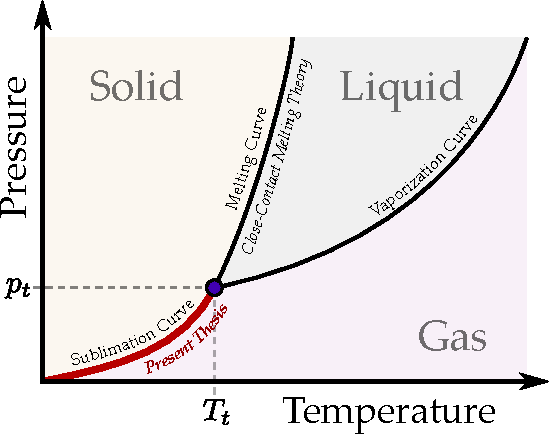
\includegraphics[trim=0 0 0 0 cm,clip,width=0.6\textwidth]{Chapters/Review/figs/phasechange/phasechange.pdf}
\caption[Simplified Phase Diagram]{Qualitative phase diagram for the subcritical regime of a substance with no phase anomaly. We recall that the type of phase transition for a pure substance depends on its temperature $T$ and pressure $p$. At the triple point $\qty(p_t, T_t)$, marked by the blue dot, all three phases (\textit{solid}, \textit{liquid}, \textit{gas}) are in thermodynamic equilibrium. The existing close-contact melting theory \cite{schuller2017spatially}, \cite{schuller2016curvilinearccm} covers solid-liquid phase transitions. This thesis extends the close-contact theory to low-pressure environments ($p < p_t$), where solid-gas sublimation occurs. \textit{This does not include the regime close to the triple point, where hybrid melting and sublimation could occur.}}
\label{fig:phasediagram}
\end{figure}

In the following, we assume pure sublimation, excluding the hybrid regime of partial sublimation and partial melting in a lid under conditions near the triple point. The latter case is also deliberately excluded from Fig. \ref{fig:ccmcworkflow}.

While the sublimation flow's mathematical description changes by dropping the assumption of incompressibility, major parts of the algorithm are straightforward extensions of the ideas developed for incompressible melts (\textbf{II} in Fig. \ref{fig:ccmcworkflow}).
In the first section of this chapter (Sec. \ref{sec:incompccm}), we will thus present a brief review of the incompressible theory, corresponding to a phase transition across the melting curve depicted in Fig. \ref{fig:phasediagram}. Special emphasis is put on the results presented in \cite{schuller2017spatially}, \cite{schuller2019icarus} and \cite{schuller2016curvilinearccm}, upon which we build the compressible theory presented in Chapter \ref{chap:compressible}.

It is theoretically possible to model the sublimation film using the full system of compressible \textit{Navier-Stokes} equations but this approach comes at a high expense of both computational and model complexity. As in the case of close-contact melting, the governing equations can however be simplified after considering a scaling described by \textit{compressible lubrication theory} (\textbf{I}). The scaled equations and simplifying assumptions are shown in Section \ref{sec:complubricationreview}.

The large mean free path of gas can render the classical continuum model (\textbf{II a}) invalid under near-vacuum conditions.  For the transition regime of moderate Knudsen numbers, the \textit{R13} theory \cite{struchtrup2003r13derivation}, \cite{struchtrup2005macroscopic} provides a deterministic macroscopic model for the rarefied gaseous flow. The issue of gas rarefaction is reviewed in Section \ref{sec:slipreview}, where we also present the hydrodynamic limit of sublimation boundary conditions derived for the R13 model \cite{beckmann2018evaporation}. We will later extend the continuum close-contact sublimation solver with this set of boundary conditions (\textbf{II b}) as a first step towards a fully non-isothermal R13 close-contact sublimation model.

\FloatBarrier


% Jump conditions
\subsection{Jump Conditions on the Phase Change Interface}\label{sec:interfacedescription}

Since an understanding of the phase change process in general, and of the interface boundary conditions in particular, is vital for a physical model closure, we briefly review interface jump conditions derived from basic conservation laws in the following section. We discuss the  classical Stefan condition as a macroscopic jump condition and sketch the Lagrangian frame of reference used in the close-contact phase change models.

Within the scope of this thesis we treat the interface between the solid and the second phase under consideration as infinitesimally thin, such that we have either pure solid or pure gaseous/liquid substance at any given point. While this makes the mathematical description of the interface relatively straightforward, it also means that we neglect mushy phase transitions where liquid- and solid fractions play a role. 

\subsubsection{General Jump Conditions}

The following descriptions can be compared to the review in \cite{mueller1985thermodynamics} and are also discussed in the Appendix of \cite{struchtrup2017evaporation} for an evaporation problem. For incompressible flows, jump conditions have been reviewed in \cite{reitzle2019directsubli} and \cite{myers2020stefan}. A detailed discussion including the effects of curvature and a mathematically sound derivation can be found in Chapter 2 of \cite{ishii2010thermo}.

In the following, we quickly elaborate on the derivation of the interface jump conditions from the basic conservation laws, repeated here for convenience using Einstein summation:
\begin{subequations}\label{eq:convjump}
\begin{flalign}
    &\textit{Mass} \quad && \pdv{\rho}{t}+\pdv{\qty(\rho\, v_k )}{x_k} =0 & \, , \label{eq:massconvjump}\\
    &\textit{Momentum} \quad && \pdv{\qty(\rho\, v_i)}{t}+\pdv{(p_{ik}+\rho\, v_i\, v_k)}{x_k}= 0& \, ,\label{eq:momconvjump}\\
    &\textit{Energy} \quad &&  \pdv{t}\qty(\rho\, \zeta + \frac{1}{2}\rho\,\norm{\Vec{v}}^2)+\pdv{x_k}\qty[\qty(\rho \,\zeta + \frac{1}{2}\rho\,\norm{\Vec{v}}^2) \,v_k + p_{ik}\,v_i+q_k]=0 &\, .  \label{eq:energyconvjump}
\end{flalign}
\end{subequations}

Here $\rho$ is the density, $v_i$ are the components, $i\in \qty[x,\,y,\,z]$, of the velocity vector $\Vec{v}$ and $\zeta$ is the specific internal energy of the fluid. The influence of body forces and internal heat sources is neglected in Eqns. \ref{eq:convjump}.

The generalized pressure tensor $p_{ij}$ is defined as
\begin{equation}\label{eq:definepij}
    p_{ij}=p\,\delta_{ij}+\sigma_{ij}\,,
\end{equation}

where $\sigma_{ij}$ is a general deviatoric stress tensor and $p$ is the isentropic pressure. In the energy conservation Eqn. \ref{eq:energyconvjump}, $q_k$, $i\in \qty[x,\,y,\,z]$ denotes components of the heat flux $\Vec{q}$.

\begin{figure}[ht!]
\centering
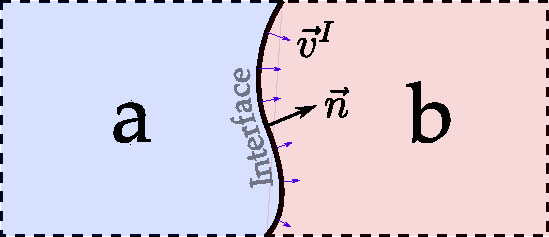
\includegraphics[trim=0 0 0 0 cm,clip,width=0.5\textwidth]{Chapters/Review/Interface/figs/discontinuity/discontinuity.pdf}
\caption[Sketch of a $2D$ Moving Interface Between Two Phases]{Sketch of a $2D$ interface with surface normal $\Vec{n}$ between two phases $a$ and $b$. The interface velocity $\Vec{v}^I$ is hinted at by the thin purple arrows. A control volume for a weak integral formulation around the interface is indicated by the dashed bounding box.} 
\label{fig:discontinuity}
\end{figure}

Figure \ref{fig:discontinuity} is a sketch of an interface between two phases $a$ and $b$ with distinct material parameters. The behavior of the discontinuity is described by \textit{jump conditions} on the interface (fat curved line). 

Macroscopic jump conditions across an interface between two phases can be derived by considering a weak integral formulation of the conservation laws (Eqns. \ref{eq:massconvjump}-\ref{eq:energyconvjump}) around the interface discontinuity. This is equivalent to the derivation of the \textit{Rankine-Hugoniot} condition routinely used in the analysis of hyperbolic PDEs. The following relations are then obtained by letting the control volume's distance from the discontinuity tend to zero \cite{myers2020stefan}:
\begin{subequations}\label{subeq:jumps}
\begin{flalign}
    & \textit{From Mass-Conservation} &&   \qty[ \rho\,\qty(v_j-v_j^I) ]_{a}^{b}\,n_j = 0\,, & \label{eq:generaljumpmass}\\
    & \textit{From Momentum-Conservation} &&   \qty[ \rho\,v_i\qty(v_j-v_j^I) + p_{ij} ]_{a}^{b}\,n_j = 0\,, & \label{eq:generaljumpmom}\\
    & \textit{From Energy-Conservation} &&\qty[ \rho\left(\zeta+\frac{\norm{\Vec{v}}^2}{2} \right)\,\qty(v_j-v_j^I)+p_{ij}\,v_i+q_j ]_{a}^{b}\,n_j = 0  \quad . \label{eq:generaljumpenergy}
\end{flalign}
\end{subequations}

% \begin{subequations}\label{subeq:jumps}
% \begin{equation}\label{eq:generaljumpmass}
%   \qty[ \rho\,\qty(v_j-v_j^I) ]_{a}^{b}\,n_j = 0\,,
% \end{equation}
% \begin{equation}\label{eq:generaljumpmom}
%     \qty[ \rho\,v_i\qty(v_j-v_j^I) + p_{ij} ]_{a}^{b}\,n_j = 0\,, 
% \end{equation}
% \begin{equation}\label{eq:generaljumpenergy}
%     \qty[ \rho\left(\zeta+\frac{\norm{\Vec{v}}^2}{2} \right)\,\qty(v_j-v_j^I)+p_{ij}\,v_i+q_j ]_{a}^{b}\,n_j = 0\quad .
% \end{equation}
% \end{subequations}



The bracket notation $\fat[ \bullet \fat]_{a}^{b}$ is introduced to describe a jump in quantity $\bullet$ across the interface from phase $a$ to $b$ where $n_i,\,i\in\{x,y,z\}$, is the local interface normal pointing from $a$ into $b$ and $v_j^I$ is the interface velocity (see Fig. \ref{fig:discontinuity}).  The variables $\rho, v_j$ and $q_j$ are the density, velocity- and heat flux components at either side of the interface respectively, $\zeta$ denotes the specific internal energy. \textit{We use the non-canonical symbol $\zeta$ to avoid confusion with the horizontal velocity component $u=v_x$ and the lubrication parameter $\epsilon$}.

Equations \ref{eq:generaljumpmass}-\ref{eq:generaljumpenergy} simply state that mass, momentum, and energy also have to be conserved across the \gls{PCI}. In the context of our close-contact model, we can use these relations as part of a mathematical closure if we have partial information about the state in either of the two phases involved. 


\subsubsection{Reference Frame}\label{sec:referenceframe}

While the jump Conditions \ref{eq:generaljumpmass}-\ref{eq:generaljumpenergy} hold in an arbitrary reference frame, a particular frame has to be decided on for a concrete problem at hand. To make the problem setup of the close-contact phase change setting introduced in Section \ref{sec:incompccm} more accessible and to avoid confusion with the analysis of the classical Stefan problem, we give a quick summary of two important frames of reference. We also establish a notation for the phase states on the interface, which will be used routinely in equations throughout this thesis. 


\begin{figure}[ht!]
    \centering
    
    \begin{subfigure}[c]{0.49\textwidth}
    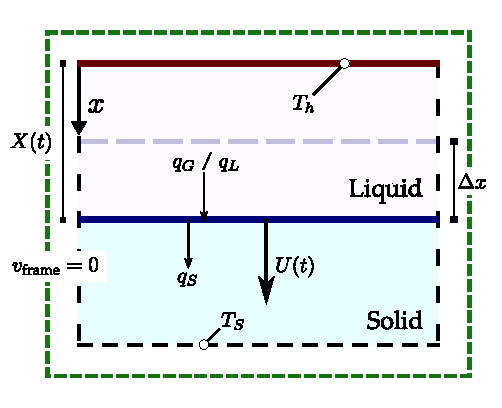
\includegraphics[trim={0cm 0.0cm 0.0cm 0.0cm},width=1\linewidth]{Chapters/Review/Interface/figs/frameofref/eulerian/stefanproblemEulerianNoArrow.pdf}
    \subcaption{Eulerian Stefan Problem}
    \label{subfig:eulerian}
    \end{subfigure}
    \begin{subfigure}[c]{0.49\textwidth}
    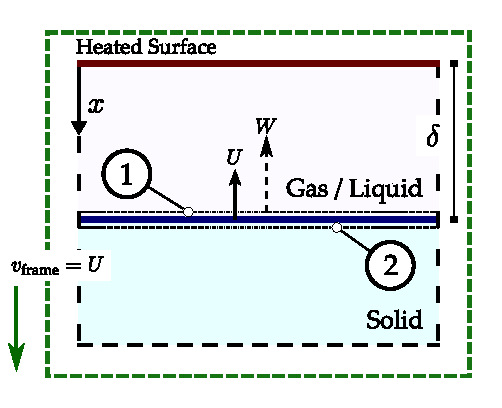
\includegraphics[trim={0.0cm 0.0cm 0.0cm 0.0cm},width=1\linewidth]{Chapters/Review/Interface/figs/frameofref/lagrangian/stefanproblemLagrangian.pdf}
    \subcaption{Lagrangian Equilibrium Phase Change}
     \label{subfig:lagrangian}
    \end{subfigure}
    
    \caption[Reference Frames for a Moving Interface Problem]{One-dimensional moving interface problem in an \textbf{Eulerian} (\textit{left}) and \textbf{Lagrangian} (\textit{right}) frame of reference. In the classical \textbf{Eulerian} view of the Stefan problem, the observer is at rest ($v\ts{frame}\equiv 0$). Driven by the heat flux induced by a heat source at $x=0$, the interface at location $X(t)$ moves with a velocity $U(t) = \partial{X}/\partial{t}$, such that an interface displacement $\Delta x$ is observed over any time span $\Delta t$. The theory of (equilibrium) close-contact melting makes use of a \textbf{Lagrangian} frame of reference, moving with the equilibrium melting velocity $v\ts{frame}=U$ (\textit{right}). Since the process is in equilibrium, $U$ is fixed for a given set of inputs (effective force and heating power). For the description of the gas/liquid flow, the interface at $X=\delta$ is treated as an inflow boundary. The velocity $W$ denotes the effective inflow velocity  of the gas or liquid, which differs from $U$ due to the change in density across the interface. The two states $\mbox{\textcircled{\tiny 1}}$ and $\mbox{\textcircled{\tiny 2}}$ refer to the two phases at infinitesimal distance from the \gls{PCI}. }
    \label{fig:referenceframes}
\end{figure}

Figure \ref{fig:referenceframes} depicts two sketches of one-dimensional moving interface problems. We distinguish between an \textit{Eulerian} or fixed reference frame (Fig. \ref{subfig:eulerian}) and a moving \textit{Lagrangian} reference frame tracing the interface movement (Fig. \ref{subfig:lagrangian}).

The Eulerian frame (Fig. \ref{subfig:eulerian}) is commonly employed in the analysis of the classical Stefan problem (Sec. \ref{sec:stefanproblem}). The frame of reference (dashed green bounding box) is static ($v\ts{frame}\equiv 0$), as is the constant-temperature heat source located at $x=0$. The interface location $X(t)$ at time $t$ moves with a velocity $U(t)$ "into" the static solid phase such that a displacement $\Delta x$ is observed. The \textit{Stefan condition} gives a relation between the interfacial heat flux $q\ts{phase}$ in the two phases and the interface velocity $U(t)$.

In the analysis of close-contact melting or sublimation problems shown in this thesis, we consider a \textit{Lagrangian} frame of reference (Fig. \ref{subfig:lagrangian}). The observer is moving with the interface ($v\ts{frame}=U$) and the origin of the coordinate system is again placed on the heater surface ($x=0$). In equilibrium, the interface is located at a constant distance $X(t)=X=\delta$ from the boundary, relative to the moving observer. 
Because the interface seems to be "at rest" at $X=\delta$ in the Lagrangian view, this particular choice of a moving reference frame may lead to the wrong conclusion that the system does not undergo active phase change on the interface. The observation that the interface is not moving relative to a moving observer or heat source does however \textbf{not} imply that no mass is exchanged between phases.

To differentiate between the observed velocity $\Vec{v}_I=\Vec{U}$ of the interface in a given reference frame, the velocity of the two phases observed on the interface and the effective velocity of melting or sublimation, we introduce the \textit{Stefan} velocity $v\ts{Stefan}$. From condition \ref{eq:massconvjump}, we formulate mass conservation across the interface between phases $a$ and $b$ as
\begin{equation}\label{eq:massjumpexample}
    \rho_a\qty(\Vec{v}_a-\Vec{v}^I)\,\Vec{n} = \rho_b\qty(\Vec{v}_b-\Vec{v}^I)\,\Vec{n}\quad . 
\end{equation}

Again, all velocities are relative to the observer. Consider now the case of close-contact solid-gas phase change, which we have introduced in Fig \ref{subfig:lagrangian}. Since the frame is moving along with the interface, we have $v^I = U-v\ts{frame}=0$. For the static solid (subscript $S$) we find $v_S= 0 - v\ts{frame} = -U$ to be the velocity relative to the observer. Eqn. \ref{eq:massjumpexample} then yields
\begin{equation}\label{eq:massjumpgassolid}
    \rho_S\underbrace{\qty(v\ts{Solid}-v\ts{frame})}_{\eqqcolon v\ts{Stefan} = -U} = \rho_G\,\underbrace{\qty(v_{L/G}-\cancel{v^I})}_{\eqqcolon W} \quad ,  
\end{equation}

where we used the subscript $L/G$ for the liquid or gaseous state  $\mbox{\textcircled{\tiny 1}}$ in Fig. \ref{subfig:lagrangian}. 

The Stefan velocity $v\ts{Stefan}$ is independent of the reference in the sense that no mass is transferred between the two phases if $v\ts{Stefan}\equiv 0$. For the two-phase melting and sublimation problems discussed in this thesis $v\ts{Stefan}$ can also be interpreted as the velocity at which a melting probe penetrates a solid icy environment.

The velocity $W\coloneqq v_{L/G}$ corresponds to the liquid or gas velocity on the \gls{PCI}. In a Lagrangian computational domain, $W$ is an inflow boundary condition for the flow in the melt- or sublimation film.
From Eqn. \ref{eq:massjumpgassolid} we find that the inflow velocity $W$ (sketched with an upward pointing arrow in Fig. \ref{subfig:lagrangian}) is related to $v\ts{Stefan}$ through
\begin{equation} \label{eq:densityboundary}
    W = v_{L/G} = \Vec{v}_{L/G}\cdot\Vec{n}\Bigg\rvert_{z=\delta} = \frac{\rho_S}{\rho_{L/G}}\, v\ts{Stefan} = -\frac{\rho_S}{\rho_{L/G}}\, U \quad .
\end{equation}

Note that for melting the second phase is liquid ($\rho_{L/G} = \rho_L$), for sublimation it is gaseous ($\rho_{L/G} = \rho_G$).

The density fraction in Eqn. \ref{eq:densityboundary} is constant as long as the density in both phases is assumed to be constant, making the boundary condition straightforward to evaluate. In particular, we have $W\approx -U$ if $\rho_b \approx \rho_a$, an assumption made for example in \cite{schuller2016curvilinearccm}, but certainly not reasonable for solid-gas phase change, where the density of solid and gas can differ by several orders of magnitude. Note that in this case, all velocities are scalar, due to the $1D$-nature of our introductory example. 

All velocities (movement of the interface and velocities in the two phases) are given relative to an observer whose movement is described by a velocity $v\ts{frame}$. 

In the following, we make two assumptions:
\begin{itemize}
    \begin{framed}
    \item We consider a Lagrangian reference frame moving with the interface, $v\ts{frame}=U$, as shown in Fig. \ref{subfig:lagrangian}.
    \item The non-negligible density difference between solid and gaseous phase in sublimation phase change enters as an inflow boundary condition in Eqn. \ref{eq:densityboundary}. For the same interface propagation speed $U$, the gas inflow velocity can subsequently be expected to have a much higher magnitude than its liquid counterpart in close-contact melting.
    \end{framed}
\end{itemize}


\subsubsection{The Stefan Problem}\label{sec:stefanproblem}

In the previous section, we introduced the Lagrangian frame of reference moving with the Stefan velocity $U = \pdv{X}{t}$. Since $U$ is unknown a priori, we need a closure relation between the states in the two phases and the propagation speed $U$ of the interface.

Since the existing close-contact melting theory, as well as the classical \textit{Stefan} theory, consider a melting process, we begin with a review of the \textit{Stefan} condition on a liquid-solid interface. We then proceed to contextualize this condition as a special case of generalized macroscopic jump conditions on an interface discontinuity between two phases. We review the general jump conditions to gain a better understanding of the physical parameters influencing the phase change boundary conditions in sublimation phase change.

\paragraph{Stefan Condition}

In the following, we review the Stefan condition which will gain importance as a boundary condition for the close-contact phase change models presented in this thesis. We start by sketching the classical Stefan problem and then show how the Stefan condition can be derived from conservation laws.

The $1D$ Stefan problem \cite{stefan1891theorie} considers a transient phase change process in which a solid at constant temperature changes into a liquid state under the influence of a heated boundary at constant temperature $T_h$. This corresponds to the configuration sketched in Fig. \ref{subfig:eulerian}, with the interface at melting temperature $T_m$ and location $x=X(t)$ propagating into the solid with velocity $U\equiv \partial X / \partial t$. 

The Stefan condition describes the conservation of energy across the interface in an arbitrary frame of reference. It relates the translation velocity $U = U(t)$ of the phase change interface (\gls{PCI}) between the two phases with the heat fluxes at the liquid ($q_L$) and solid ($q_S$) side of the interface:
\begin{equation}\label{eq:1dstefan}
    \rho\, h_m \underbrace{\pdv{X}{t}}_{U\equiv}  = -\kappa_L \pdv{T(X(t),t)}{x}\bigg\rvert_{\mathbf{X}^-} + \kappa_S \pdv{T(X(t),t)}{x}\bigg\rvert_{\mathbf{X}^+} \equiv q_L - q_S \quad ,
\end{equation}

where $\kappa_L$ and $\kappa_S$ denote the thermal conductivities of liquid and solid phase respectively and  $\mathbf{X}^\pm \coloneqq \lim_{h\to 0}X(t)\pm h$. In the context of equilibrium melting and sublimation, we will usually call the interface location relative to a heat source \textit{film thickness} $\delta = X$. 

Knowledge about the solid heat flux $q_S$ is required to close the models presented in this thesis. A common approximation in equilibrium melting (or sublimation) is to assume an equilibrium velocity $U$, resulting in a stationary temperature profile in the solid domain \cite{schuller2017spatially}. This was also sketched in (\textbf{a}) of the introductory Fig. \ref{fig:introEquilibria}. The flux $q_S$ can then be found from the analytical solution of a $1D$ steady advection-diffusion boundary value problem in the solid domain to yield
\begin{equation}\label{eq:qsflux}
    q_{S}=\rho_S \,c_{p,S}\, U\,(T_m-T_S)\,.
\end{equation}

Here, $\rho_S$ and $c_{p,S}$ are the solid density and heat capacity respectively. $T_S$ is the solid far field temperature $T_S= T(x\to\infty)$.

The Stefan condition from Eqn. \ref{eq:1dstefan} can then be rewritten in terms of the flux at the liquid boundary $q_L$:

\begin{equation}\label{eq:qlequilibrium}
    q_L = \rho_S \, U\,(h_m + \frac{q_S}{\rho_S\,U}) \overset{\ref{eq:qsflux}}{=} \rho_S \, U\,\underbrace{(h_m + c_{p,S}(T_m-T_S)\,)}_{\text{reduced latent heat }h_m^*}\,.
\end{equation}

Note that the Stefan condition also generalizes to multiple dimensions where the normal heat flux can still be computed from an inner product of temperature gradients with the interface normal vector. For the two-dimensional approximations of the melt film discussed in this thesis, we can assume the interface location $\delta$ to remain approximately constant across the \gls{PCI}, as long as the boundary condition on the heat source surface is a constant. In this case, the interface condition again simplifies to Eqn. \ref{eq:1dstefan}.

\paragraph{Relation to General Jump Conditions}
 We now contextualize the \textit{Stefan} condition as a special case of the generalized energy conservation (Eqn. \ref{eq:generaljumpenergy}) across the interface. We also argue to neglect the interfacial pressure jump in the absence of curvature effects, closely following arguments from Section 1.2.3 of \cite{ishii2010thermo}. This summary again considers the two-phase scenario introduced in the previous section and sketched in Fig. \ref{fig:discontinuity}. 

The following perspective on interface jump condition is useful to quantify which physical influences are neglected by relying on the classical Stefan closure \ref{eq:1dstefan}, even more so if we extend the model for solid-liquid melting to simulate sublimation phase change. 

We emphasize again that the interface is taken to be infinitesimally thin the derivation of Eqns. \ref{eq:generaljumpmass}-\ref{eq:generaljumpenergy} and a fully reversible process is considered. This means that the entropy production of the interface is zero and the interfacial entropy inequality can be used to infer simplified boundary conditions on the \gls{PCI}. The argument can be followed in more detail in Chapter 2 of \cite{ishii2010thermo}, we restrict ourselves to a review of the most important boundary conditions used in this thesis. 

The first important boundary condition concerns the temperature on the interface. Assuming zero entropy production at the interface, one arrives at \cite{ishii2010thermo}
\begin{equation}\label{eq:assumetsat}
    T^a = T^b = T\ts{sat} \quad ,
\end{equation}

which is routinely used in the analysis of two-phase problems. 

Under this assumption, the relationship between the saturation curve $p\ts{sat}(T\ts{sat})$ and the real interface pressure is depicted in Fig. \ref{fig:dpsaturationcurve}. The saturation curve (\textbf{solid black line}) marks the condition of equilibrium between phases \textbf{a} and \textbf{b}. For an interface at rest ($\mbox{\textcircled{\tiny 1}}$, \textit{left}) the temperatures and pressures in both phases agree with a point $\qty(T_{i,1}=T\ts{sat,1},\,p\ts{sat}(T_{i,1}))$  on the sublimation curve. For a moving interface ($\mbox{\textcircled{\tiny 2}}$, \textit{right}), pressures $p^a$ and $p^b$ generally differ from $p\ts{sat}(T_{i,2})$. The real interface pressure in each phase then lies somewhere in a range between the saturation pressure and some limit $p\ts{max}$ /$p\ts{min}$, indicated by the dotted lines.  



\begin{figure}[ht!]
\centering
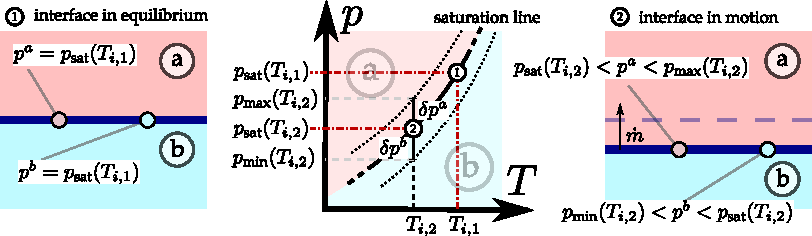
\includegraphics[trim=0 0 0 0 cm,clip,width=1\textwidth]{Chapters/Review/Interface/figs/satcurve/interfaceconditions.pdf}
\caption[Saturation Curve and Pressure Jump]{Relation between the saturation line $p\ts{sat}(T)$ (\textit{solid black line}) and the pressure on an interface between phases \textbf{a} and \textbf{b}. The sketches show an interface in equilibrium  ($\mbox{\textcircled{\tiny 1}}$, \textit{left}) at which the pressure in both phases corresponds to a point $p\ts{sat}(T_{i,1})$ exactly on the saturation curve. This is not generally true for a non-equilibrium interface ($\mbox{\textcircled{\tiny 2}}$, \textit{right}). A theoretical limit for the existence of phase \textbf{a} and \textbf{b} is hinted at by the \textit{dotted black lines}. \textit{This figure is an extension of \textit{Fig. 2-3} in \cite{ishii2010thermo}}.} 
\label{fig:dpsaturationcurve}
\end{figure}


Eqn.\ref{eq:momconvjump} can be manipulated to find an explicit expression for the interface pressure jump $\qty[p]_a^b$:
\begin{align}
    \qty[p]_a^b \coloneqq p^b-p^a \stackrel{}{=} &
    \rho^a\,v^a_n\,\qty(v^a_n-v^I_n) - \rho^b\,v^b_n\,\qty(v^b_n-v^I_n)  -\qty(\vect{\sigma}^b_n-\vect{\sigma}^a_n) \cdot \vect{n} \notag \\ 
    \stackrel{}{=} & 
    \qty(\frac{\rho^b}{\rho^a})\underbrace{\qty(\rho_b - \rho_a)}_{\coloneqq \qty[\rho]_a^b}
    \,\qty(v^I_n-v^b_n)^2 -\underbrace{\qty(\vect{\sigma}^b_n-\vect{\sigma}^a_n)}_{\coloneqq \qty[\vect{\sigma}_n]_a^b} \cdot \vect{n} \notag\\
    = & 
    \qty(\frac{\rho^b}{\rho^a})\qty[\rho]_a^b
    \,\qty(v^I_n-v^b_n)^2 - \qty[\vect{\sigma}_n]_a^b \cdot \vect{n}\quad . \label{eq:pressurejumpcond}
\end{align}

For the ease of notation, we define the scalar $v^\bullet_n \coloneqq \vect{v}^\bullet\cdot\vect{n}$ and vector  $\vect{\sigma}^\bullet_n \coloneqq \matr{\sigma}^\bullet\cdot\vect{n} = \sigma_{ij}^\bullet\,n_j$ that occur as inner products with the interface normal.

Moreover, neglecting stress contributions, Eqn. \ref{eq:pressurejumpcond} can be expressed in terms of the interfacial mass flux  
\begin{equation*}
    \Dot{m}=\rho_k\,\qty(v^k_n-v^I_n) = \rho_G\,W = -\rho_S\,U
\end{equation*}
as
\begin{equation}
    \qty[p]_a^b \approx \qty(\frac{1}{\rho^a}-\frac{1}{\rho^b})\,\qty(\rho^b)^2\,\
    \,\qty(v^I_n-v^b_n)^2  = \qty(\frac{1}{\rho^a}-\frac{1}{\rho^b})\,\Dot{m}^2 \quad . \notag
\end{equation}

As discussed in detail in Section 1.2.3 of \cite{ishii2010thermo}, normal stress contributions are typically negligible, such that Eqn. \ref{eq:pressurejumpcond} is a reasonable approximation of the pressure jump across the interface if curvature effects play no role. We follow the argument of \cite{ishii2010thermo}, using Eqn. \ref{eq:pressurejumpcond} to argue that it is valid to assume $\qty[p]_a^b \approx 0$ for typical sublimation mass flow rates. This leads to the simplified condition
\begin{equation}\label{eq:psatassumption}
    p^a = p^b = p\ts{sat}(T^I)\quad ,
\end{equation}
meaning that the pressure in both phases equals the equilibrium saturation pressure $p\ts{sat}(T^I)$ at the interface temperature $T^I$ under the aforementioned assumptions.

A similar analysis can finally be conducted for the energy jump condition (Eqn. \ref{eq:generaljumpenergy}). Inserting the definition of the pressure tensor $p_{ij}$ (Eqn. \ref{eq:definepij}), replacing the specific internal energy $\zeta$ with the specific enthalpy $h$ defined as 
\begin{equation}
    h = \zeta + \frac{p}{\rho} \, \Rightarrow  \zeta = h - \frac{p}{\rho}
\end{equation}

and introducing the total specific enthalpy
\begin{equation}
   h\ts{tot}=h+e\ts{kin}= h+\norm{\vect{v}}^2/2 \quad ,
\end{equation}

Eqn. \ref{eq:generaljumpenergy} can be rewritten as
\begin{align}
    \rho_b\underbrace{\qty( h\ts{tot}^b - h\ts{tot}^a)}_{\qty[h\ts{tot}]_a^b}\,\qty(v^I_n-v^b_n)
    & = \underbrace{\qty(p^b-p^a)}_{\qty[p]_a^b}\,v^I_n 
    + \underbrace{\qty(q^b_n-q^a_n)}_{\qty[\vect{q}]_a^b\cdot\vect{n}}
    + \underbrace{\qty(\matr{\sigma}^b\,\vect{v}^b
    -\matr{\sigma}^a\,\vect{v}^a)}_{\qty[\matr{\sigma}\,\vect{v}]_a^b}\cdot \vect{n} \notag \\
    \rho_b\qty[h\ts{tot}]_a^b\,\qty(v^I_n-v^b_n)
    &=\qty[p]_a^b\,v^I_n 
    + \qty[\vect{q}]_a^b\cdot\vect{n}
    + \qty[\matr{\sigma}\,\vect{v}]_a^b \cdot \vect{n} \label{eq:energyjumpfinalreview}\quad .
\end{align}

In symmetric form this reads
\begin{equation}
    -m\,\qty[h\ts{tot}]_a^b=\qty[p]_a^b\,v^I_n 
    + \qty[q_n]_a^b
    + \qty[\matr{\sigma}\,\vect{v}]_a^b \cdot \vect{n}\,,
\end{equation}

after inserting the interfacial mass flux $m \coloneqq \rho_b\,\qty(v^b_n-v^I_n) = \rho_a \qty(v^a_n-v^I_n)$.

In the context of phase change problems, we can define
\begin{equation}
    U \coloneqq v_j^I \,n_j = \vect{v}^I \cdot \vect{n} = v^I_n
\end{equation}

as the velocity of melting, evaporation, or \textit{sublimation} depending on the phases involved. In the classical \textit{Stefan} melting theory \cite{stefan1891theorie}, a solid-liquid interface is considered ($a=S$ and $b=L$ for solid and liquid phase respectively). 

As discussed in Section 2.3 of \cite{myers2020stefan}, the contribution of kinetic energy  to the total enthalpy density 
\begin{equation}
     h\ts{tot}= h+ \underbrace{\cancel{\norm{\vect{v}}^2/2}}_{\textit{neglect}} \approx h \, ,\notag
\end{equation}
is commonly neglected, since it is assumed to be negligible compared to the latent heat. If curvature effects play no role and the velocity $v^L_n$ on the liquid side of the boundary is small enough, it is furthermore reasonable to neglect the stress flux term $\qty[\matr{\sigma}\,\vect{v}]_a^b \cdot \vect{n}$. 

In this case, we recover the Stefan condition from Eqn. (\ref{eq:energyjumpfinalreview}) since
\begin{align}
    & 
    \rho_S\qty[h]_S^L\,\qty(\cancel{v^I_n}-v^S_n) = -\rho_S\qty[h]_S^L\,U 
    =\qty[p]_S^L\,\underbrace{\cancel{v^I_n}}_{(C)} 
    + \qty[\vect{q}]_S^L\cdot\vect{n}
    + \underbrace{\cancel{\qty[\matr{\sigma}\,\vect{v}]_S^L \cdot \vect{n}}}_{\text{neglect}} \notag\\
    \Rightarrow \quad &
    \qty[\vect{q}]_{L}^{S}\cdot \vect{n} 
    = \rho_S\,\qty[ h ]_{L}^{S}\, \vect{v}^I\cdot \vect{n} = \rho_S \, h_m \,U\, \quad . \label{eq:stefancondition}
\end{align}

 Here, $h_m =\qty[ h ]_{L}^{S} $ is the specific latent heat of melting. Note that the observed interface normal velocity $v^I_n$ is zero due to the choice of a reference frame moving with the same velocity. In an arbitrary reference frame, the influence of the pressure jump $ \qty[p]_a^b$ can be assessed by evaluating Eqn. \ref{eq:pressurejumpcond} or neglected following the argument leading up to Eqn. \ref{eq:psatassumption}. 
 
 The above review can be summarized:
 \begin{itemize}
     \begin{framed}
     \item Assuming zero-entropy production on the interface, one can infer $T_G = T_S = T\ts{sat}$. This will be used as a Dirichlet boundary condition on the solid-gas sublimation interface in the continuum model (Chapter \ref{chap:compressible}). 
     \item Neglecting curvature effects we arrived at an equivalent simplification for the interface pressure, $p_G= p_S = p\ts{sat}$.
     \item The Stefan condition can be contextualized as a special case of general energy conservation across the interface. In particular we neglect stress contributions by assuming the simple form shown in Eqns. \ref{eq:1dstefan} and \ref{eq:stefancondition}. This relation is later used as a closure condition to find the equilibrium film thickness $\delta$.
     \end{framed}
 \end{itemize}
 
 
 






% Incompressible CCM
\subsection{Incompressible Close-Contact Melting}\label{sec:incompccm}

The theory of close-contact melting is occupied with the analysis of phase change processes that are induced by a heat source separated from a solid \textit{ phase change material} by a very thin liquid layer (\textit{melt film}). In the following section we review findings from \cite{schuller2017spatially}, \cite{schuller2019icarus}, \cite{schuller2016curvilinearccm} which the compressible solver proposed in this thesis builds upon.

For the solid-liquid phase change considered in simulations of melting it is natural to assume incompressibility in the liquid phase, granting analytical access to the description of the $2D$ flow field. However, one goal of this thesis is to quantify the influence of compressibility effects. While the computational complexity of the solution strategy for ideal gas sublimation flow proposed in Chapter \ref{chap:compressible} increases compared to the incompressible theory reviewed in the following, it is conceptually based on the incompressible close-contact solvers described in \cite{schuller2017spatially} and \cite{schuller2016curvilinearccm}. 

The incompressible \gls{CCM} thus lends itself to a first introduction to the problem configuration.  By emphasizing key differences between incompressible melting and compressible sublimation, we hope to grant easier access to the derivations in Chapter \ref{chap:compressible}.

Special emphasis is put on the cylindrical configuration presented in \cite{schuller2019icarus} since it will be used as a reference geometry in our simulations of sublimation phase change. 

\subsubsection{Problem Description}
In the following we consider a two-dimensional close-contact melting process in cylindrical coordinates.

Figure \ref{fig:ccmsetupsketch} is a recreation of the configuration discussed in \cite{schuller2019icarus}. It shows a sketch of a close-contact melting problem with a cylindrical, axisymmetric heater of diameter $L$, separated from the solid phase by the melt film of thickness $\delta \ll L$. The phase change interface $\Gamma_C$ (\gls{PCI}) located at $z=\delta$ advances with a velocity $U$ relative to the static icy environment, a process driven by the additition of heat through the heater surface $\Gamma_H$ ($z=0$). The Lagrangian frame of reference employed in the theoretical analysis of the system presented in Figure \ref{fig:ccmsetupsketch} has been reviewed in the previous Section \ref{sec:interfacedescription}.

In equilibrium melting, the contact force induced by the pressure distribution across the melt film is in balance with the external, buoyancy correct force 
\begin{equation} \label{eq:feffective}
    F\ts{eff} = F\ts{g} - \rho_L\,V\ts{probe}\,g \quad .
\end{equation}

Here, $F\ts{g}$ is the graviational force acting on the probe, $\rho_L$ is the (constant) liquid density and $g$ is the gravitational acceleration. $V\ts{probe}$ is the volume of the probe, which equals $V\ts{probe}=\pi\,L^2\,H$ for a cylindrical melting head of radius $L$ and height $H$. Another important implication of \textit{equilibrium} melting is that the melt film thickness or distance of the phase change interface from the heater surface $\delta$, as well as the interface propagation speed $U$ relative to the ice at rest, remain constant. This means that the flow and heat transfer processes in the melt film can be considered stationary, even though the probe itself is moving. This is shown in the introductory Figure \ref{fig:introEquilibria}, where temperature profile (\textit{left}) and pressure distribution (\textit{right}) are depicted in an equilibrium melt film.




\begin{figure}[ht!]
\centering
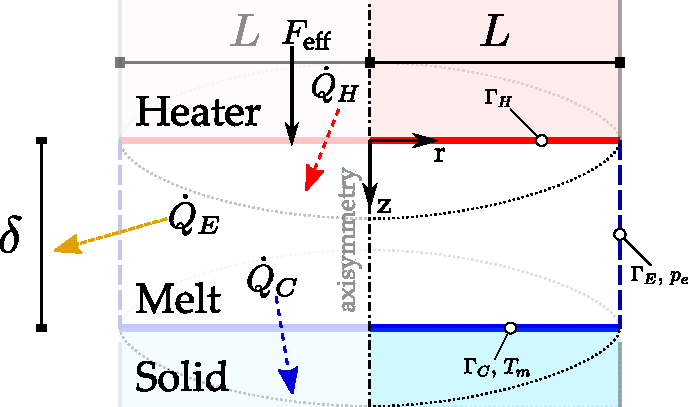
\includegraphics[trim=0 0 0 0 cm,clip,width=0.7\textwidth]{Chapters/Review/CCM/figs/cylindersketch/cylindersketch.pdf}
\caption[Close-Contact Melting: Problem Statement]{Problem description of a (cylindrical) close-contact melting problem. As heat is added through the heater surface $\Gamma_H$, a melt film of thickness $\delta$ separates the solid-liquid phase change interface (\gls{PCI}) $\Gamma_C$ from the heater. Note that the figure displays an axisymmetric cylindrical geometry with the axis of symmetry located at $r=0$. The symmetry is hinted at by the figure's brightness, the cylinder has the radius $L$. A constant pressure $p_e$ is assumed at the outflow boundary $\Gamma_E$. The simplified heat balance, sketched using the dashed arrows on the left half of the figure, distinguishes between a heat flux $\Dot{Q}_H$ induced by the heater, a heat flux $\Dot{Q}_C$ driving the phase change process and the outflux $\Dot{Q}_E$ leaving the system through the lateral outflow. \textit{Note that the Figure's aspect ratio is \textbf{not to scale} for better visibility.}} 
\label{fig:ccmsetupsketch}
\end{figure}


\subsubsection{Governing Equations in Cylindrical Coordinates}

While different phase change materials and heater geometries have been studied, all investigations rely on the common assumption that the film thickness $\delta$ is negligible compared to the heater's extensions in the other dimensions, e.g. $\delta \ll L$ or $\epsilon \coloneqq \delta / L\ll 1$ for the $2D$ case discussed here. In a Lagrangian frame of reference, tracking the interface (see Section \ref{fig:ccminterfacegeometry}), incompressible lubrication theory  \cite{hamrock2004fundamentalslubrication} then yields the following governing equations,
\begin{subequations}\label{eq:governingccm}
\begin{flalign}
    &\textit{Conservation of Mass}\quad && \frac{1}{r}\,\pdv{\qty(r\,u)}{r} + \pdv{w}{z}  = 0 & \quad , \label{eq:massccm}\\
    &\textit{Conservation of Momentum}\quad && \mu_L\,\pdv[2]{u}{z} = \pdv{p}{r} &   \quad ,\label{eq:momccm}\\
    &\textit{Conservation of Energy}\quad && u\,\pdv{T}{r} + w\,\pdv{T}{z}  = \alpha_L\,\pdv[2]{T}{z} & \quad , \label{eq:energyccm}
\end{flalign}
\end{subequations}

on the domain $\qty(r,\,z)\in\qty[-L,L]\cross\qty[0,\,\delta]$. This simplified set of equations is valid as long as the Reynolds number $\textit{Re}=\qty(\rho_L\,U\,L)/\qty(\epsilon\,\mu_L)$ satisfies $\textit{Re}\,\epsilon^2\ll1$. In the above equations $p$ and $T$ denote the pressure and temperature in the melt film. Variables $u,\,v$ denote $r$ and $z$-components of the velocity vector $(u,\,w)=(v_r,\,v_z) = \Vec{v}^T$. The material parameters $\mu_L$ and $\alpha_L=\kappa_L / \qty(\rho_L\,c_{p,L})$ are dynamic viscosity and thermal diffusivity respectively. $\kappa$ and $c_p$ refer to the material's thermal conductivity and specific heat capacity. Capital subscripts $L$ (\textit{liquid}), $S$ (\textit{solid}) and $G$ (\textit{gas}) will be used throughout this thesis to denote a parameters' phase affiliation.

The most important consequence of the scaling result \ref{eq:governingccm} is the depth independence of pressure $p$. It is preserved even in the compressible case (see Section \ref{sec:complubricationreview}).

\subsubsection{Boundary Conditions}

To solve the system of governing Equations \ref{eq:massccm}-\ref{eq:energyccm} we require boundary conditions for pressure $p$, temperature $T$, and velocity $\qty(u,w)$. 

Note that assuming a constant film thickness $\delta$ is a simplification to avoid further technicalities in the solution procedure, especially when it comes to a parametric description and numerical discretization of a domain with variable depth.  
Figure $\ref{fig:ccminterfacegeometry}$ sketches the interface geometry for a radially symmetric melt film of variable thickness. The center-line of symmetry is indicated by a gray vertical dash-dot line.

The surface normal is then given by

\begin{equation}
    \Vec{n} = \mqty(n_r \\ n_z) = \frac{1}{\sqrt{1 + \delta'(r)}}\mqty(\delta'(r) \\ -1) \quad ,
\end{equation}

For an in-depth derivation of governing equations given a variable melt film thickness and a discretization approach using a variable transformation the reader is referred to \cite{schuller2017spatially}. Throughout this thesis we will assume $\delta(r)\equiv \delta = \textit{const}$ or $\delta'=\partial\delta / \partial r = 0$, thus $n = n_z$. 

The boundary conditions for velocity then read
\begin{subequations}\label{eq:ccmvelocityboundary}
\begin{flalign}
     &\textit{Heater Surface} && u(r,0) = 0\,, \quad &w(r,0) &= 0\,, & \\
     &\textit{Interface Mass Conservation} && u(r,\delta) = 0\,, \quad & W \coloneqq w(r, \delta) &= -\frac{\rho_S}{\rho_L}\,U & \quad .
\end{flalign}
\end{subequations}

The interface boundary conditions ($z=\delta$) for velocity are based on the mass conservation condition across the interface discussed in Section \ref{sec:interfacedescription} and depend on the particular choice of a Lagrangian reference. Recalling the previous paragraph, the mass flow across the interface takes places in $z$-direction exclusively.

Temperature boundary conditions for a process driven by a surface heat flux $\Dot{Q}_H$ read
\begin{subequations}
\begin{flalign}
     &\textit{Fourier's Law} && \pdv{T}{z}\Bigg\rvert_{z=0} = -\frac{\Dot{Q}_H}{\kappa_L\,A\ts{h}} & \quad , \label{eq:ccmtempbcfluxheater}\\
     &\textit{Interface Melting Temperature} && T(x,\,z=\delta) = T_m  & \quad , \label{eq:ccmtempbcmeltingtemp}\\
     &\textit{Interface Stefan Condition} &&  \pdv{T}{z}\Bigg\rvert_{z=\delta} = - \frac{\rho_S\,U\,h_m^*}{k_L}  &\quad . \label{eq:ccmstefan}
\end{flalign}
\end{subequations}

On the interface the temperature field $T=T(r,\,z=\delta)$ has to satisfy melting temperature $T_m$. The equilibrium melting temperature is a point on the melting curve of the phase diagram (recall Fig. \ref{fig:phasediagram}) and, in principle, a function of the pressure $p(x)$ on the interface. However,  the temperature variation $T_m(p)$ is negligible for the pressure variations occurring in real \gls{CCM} melting scenarios and thus a constant Dirichlet boundary condition is imposed.

While the pressure distribution takes on a certain boundary pressure $p_e$ at the laterals,
\begin{equation}
    p(\pm L) = p_e\quad ,
\end{equation}

it only appears as a constant in the solution of Eqn. \ref{eq:momccm}. 



\begin{figure}[ht!]
\centering
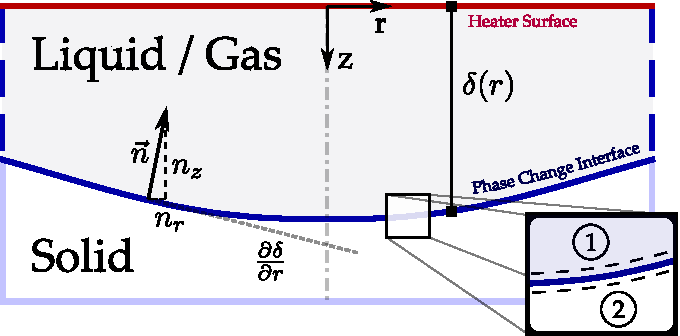
\includegraphics[trim=0 0 0 0 cm,clip,width=0.7\textwidth]{Chapters/Review/Interface/figs/interface/interfaceCylindrical.pdf}
\caption[Close-Contact Phase Change: Interface Description]{Variable thickness close-contact phase change problem. The figure illustrates the geometry of the interface parametrization $\delta(r)$ used in the description of (jump) boundary conditions on the phase change interface (\textit{solid, curved blue line}). The normal vector $\Vec{n}$ on the interface is of particular importance and sketched here at an arbitrary location on the \gls{PCI}. The direction of the surface tangent at the same position is given by $\partial\delta / \partial r$, hinted at by the dashed gray line. Note the assumed symmetry with respect to the $r=0$ center line (\textit{vertical dash-dot line}). For a given position on the interface we will formulate jump conditions in terms of the two phase's states $\mbox{\textcircled{\tiny 1}}$ and $\mbox{\textcircled{\tiny 2}}$ at infinitesimal distance from the \gls{PCI}.} 
\label{fig:ccminterfacegeometry}
\end{figure}

\subsubsection{Incompressible Solution}

The incompressible pressure profile for cylindrical close-contact can by found by algebraic manipulation of Eqns. \ref{eq:massccm}-\ref{eq:momccm} \cite{schuller2019icarus} and is given by relation 

\begin{equation}\label{eq:pincompcylinder}
    p(r) = p_e + \frac{3\,\mu_L\,W\,\qty(L^2-r^2)}{\delta^3} \quad \quad r \in \qty[-L,L] \quad ,
\end{equation}

with (constant) interface fluid velocity $W$ related to the Stefan velocity $U$ by $W = \qty(\rho_S / \rho_L)\, U$ (Eqn. \ref{eq:ccmvelocityboundary}). 

The horizontal and vertical velocity components $u$ and $w$ are then found from
\begin{subequations}\label{eq:incompccmvelocity}
\begin{flalign} 
    \qquad \qquad & u(r,z) = -\frac{6\,r\,\mu_L\,W\,r\,z\,\qty(z-\delta)}{\delta^3} & \quad \qty(r,\,z)\in \qty[-L,\,L]\cross\qty[0,\,\delta] \quad ,\\
    \qquad \qquad &  w(r,z) = \frac{6\,W}{\delta^3}\,\qty(\frac{z^3}{3} - \frac{z^2}{2}\,\delta) & \quad \qty(r,\,z)\in \qty[-L,\,L]\cross\qty[0,\,\delta] \quad .
\end{flalign}
\end{subequations}

% \begin{equation} \label{eq:incompressibleheat}
%     \rho_L\,c_{p,L} \, \qty(u\,\pdv{T}{x} + w\,\pdv{T}{z}) = \kappa_L \, \pdv[2]{T}{z} \quad \quad \quad\quad \qty(r,\,z)\in \qty[-L,\,L]\cross\qty[0,\,\delta] 
% \end{equation}

Instead of numerically solving the incompressible heat Equation \ref{eq:energyccm} across the melt, the authors of \cite{schuller2019icarus} propose to prescribe a quadractic $1D$ polynomial that satisfies the heating flux boundary condition at $z=0$ (Eqn. \ref{eq:ccmtempbcfluxheater}) and the melting temperature and Stefan condition on the \gls{PCI}, $z=\delta$ (Eqns. \ref{eq:ccmtempbcmeltingtemp} and \ref{eq:ccmstefan}). Using the three boundary conditions to solve for the polynomial's coefficients one obtains 
\begin{equation}\label{eq:temperaturequadraticreview}
    T(r,z) = \frac{\Dot{q}_H - \rho_S\,U\,h_m^*}{2\,\delta\,\kappa_L}\,\qty(z^2-\delta^2) + \frac{\Dot{q}_H}{\kappa_L}\,\qty(\delta - z) + T_m \quad .
\end{equation}

Here we introduced $\Dot{q}$ as our notation for the heat flux in $\Dot{q}_H=\Dot{Q}_H / A_H$, where $\Dot{Q}_H$ is the power added to the system through the heater surface ($z=0$) of area $A_H$.
As shown in the later Chapter \ref{chap:results}, Ansatz \ref{eq:temperaturequadraticreview} can indeed be validated to be an accurate approximation to the real solution of Eqn. \ref{eq:energyccm} in incompressible melting. It is however not directly clear if this result generalizes to compressible flows. 

The cylindrical contact force is readily computed by integrating the pressure over the heater surface
\begin{equation}\label{eq:ccmpressureforce}
    F_p = 2\,\pi\,\int_0^L \qty(p(\hat{r})-p_e)\,\hat{r}\, \mathrm{d}\hat{r} \quad .
\end{equation}

To evaluate Eqns. \ref{eq:incompccmvelocity} and \ref{eq:temperaturequadraticreview} one requires knowledge about the melt film thickness $\delta$. A closure relation proposed in \cite{schuller2019icarus} uses the fact that the correct equilibrium melt film thickness $\delta$ must be found such that 
\begin{enumerate}

    \item the temperature $T(r, z)$ satisfies the Stefan condition (Eqn. \ref{eq:ccmstefan}) everywhere on the interface $z=\delta$ (\textit{thermodynamic equilbrium)} and
    \item the contact force $F_p$ (Eqn. \ref{eq:ccmpressureforce}) exerted by the pressure  distribution is in balance with the effective force $F\ts{eff}$ induced by the melting probe (\textit{mechanical equilibrium}).  
\end{enumerate}

The two conditions can be used to find two independent relations for $\delta$,
\begin{subequations}
\begin{flalign}
     & \textit{from thermodynamic equilbrium } && \delta= \frac{20\,\alpha_L\,\rho_L\qty(\Dot{q}_H-\rho_S\,U\,h_m^*)}{U\,\rho_S\,\qty(3\,\Dot{q}_H + 7\,\rho_S\,U\,h_m^*)} & \quad , \label{eq:ccmdeltathermodynamic}\\
     & \textit{from mechanical equilbrium } && \delta= \qty(\frac{3}{2}\,\frac{\pi\,L^4\,\mu_L\,\frac{\rho_S}{\rho_L}\,U}{F_p - \rho_L\,V\ts{probe}\,g})^{1/3}& \quad .
\end{flalign}
\end{subequations}

The correct equilibrium melt film thickness can be found by equating the two relations above and solving for $\delta$ using a numerical root finding strategy.

In  Table \ref{tab:ccmequilibria} we summarize the role of equilibrium conditions as convergence criteria in iterative solvers for the state of an equilibrium close-contact phase change system. 
Note that this is assuming an effective force $F\ts{eff}$ as an input to the system. One can also just assume a velocity $U$. The resulting pressure distribution $p$ can then be integrated (Eqn. \ref{eq:ccmpressureforce}) to find the required force $F\ts{eff}$ to achieve a given $U$. 

\begin{table}[ht!]
\begin{tabular}{ll|
>{\columncolor[HTML]{EFEFEF}}l |l|
>{\columncolor[HTML]{ECF4FF}}l}
\textit{Equilibrium Cond.}                                                      &  & \textbf{Thermodynamical (a)}                                                              &  & {\color[HTML]{333333} \textbf{Mechanical (b)}}                                                                       \\
\textit{Iteration Variable}                                                    &  & \begin{tabular}[t]{@{}l@{}}Lubrication Film Thickness\\ $\delta$\end{tabular}  &  & {\color[HTML]{333333} \begin{tabular}[t]{@{}l@{}}Interface Prop. Speed\\ (\textit{Stefan Velocity}) $U$\end{tabular}}                         \\
                                                                               &  &                                                                                                  &  &                                                                                                       \\
\textit{\begin{tabular}[t]{@{}l@{}}Coressponding Flow\\ Property\end{tabular}} &  & \begin{tabular}[t]{@{}l@{}}Steady Temperature\\ Distribution $T(x,z)$\end{tabular}    &  & {\color[HTML]{333333} \begin{tabular}[t]{@{}l@{}}Pressure Distribution $p(x)$\\ \end{tabular}}                    \\
                                                                               &  &                                                                                                  &  &                                                                                                       \\
\textit{Macroscopic Balance}                                                   &  & \begin{tabular}[t]{@{}l@{}}Local Energy Conservation \\ at the Interface \\ (\textit{Stefan Condition}
)\end{tabular}                                                            &  & {\color[HTML]{333333} \begin{tabular}[t]{@{}l@{}}Effective Force $F\ts{eff}$\\ \end{tabular}}
\end{tabular}
\caption[Equilibrium in Close-Contact Phase Change]{Mechanical and thermal balance in close-contact phase change. Close-contact models aim to find the state of system at which (\textbf{a}) the temperature distribution satisfies the interface \textit{Stefan condition} (Eqn. \ref{eq:stefancondition}) and (\textbf{b}) the pressure distribution $p(x)$ is in balance with the effective force $F\ts{eff}$ (Eqn. \ref{eq:feffective}) exerted on the lubrication film (\textit{mechanical equilibrium}). The film thickness $\delta$ and Stefan velocity $U$ can be iterated upon, to match conditions \textbf{(a)} and \textbf{(b)} respectively.}
\label{tab:ccmequilibria}
\end{table}


\subsubsection{Energy Balance and Melting Efficiency}\label{subsec:ccmefficiency}

Following \cite{schuller2019icarus}, a very basic melt film energy balance distinguishes between three contributions
\begin{equation}
    \Dot{Q}_H - \Dot{Q}_E - \Dot{Q}_E = 0 \quad .
\end{equation}

The power $\Dot{Q}_H$ is added trough the heater surface $\Gamma_H$ with area $A_H$. This heat is split among the heat flux across the \gls{PCI}, $\Dot{q}_C=\Dot{Q}_C / A_H$, which is necessary to sustain phase change, and a loss $\Dot{q}_E$ through the lateral outflow boundary $\Gamma_E$. The control domain and the heat flow are sketched in Fig. \ref{fig:ccmsetupsketch}.

As a measure of process efficiency $\gamma$ one can now define the fraction
\begin{equation}\label{eq:defgamma}
    \gamma \coloneqq \frac{\Dot{Q}_C}{\Dot{Q}_H} = \frac{\Dot{q}_C}{\Dot{q}_H}
\end{equation}

of the total input heat used to drive the phase change process. In the limit of perfect efficiency, $\gamma = 1$, we have $\Dot{q}_C = \Dot{q}_H$ or $\Dot{q}_e = 0$, meaning that the full heating power is used to melt the ice and no convective losses occur.

The Stefan condition at the \gls{PCI} lets us rewrite Eqn. \ref{eq:defgamma} in terms of the effective Stefan velocity $U$ of the melting process. 

\begin{framed}
Recalling the Stefan condition $\Dot{q}_C = \rho_S\,U\,h_m^*$, we find an upper limit $U^*$ for the Stefan velocity at optimal efficiency ($\gamma = 1$) from
\begin{equation}\notag
     \Dot{q}_C^*  =  \rho_S\,U^*\,h_m^* \overset{\gamma = 1}{=} \Dot{q}_H \quad
    \Longleftrightarrow\quad   U^*=  \frac{\Dot{q}_H}{ \rho_S\,h_m^*}\notag \quad ,
\end{equation}
allowing us to rewrite the efficiency in terms of the velocity ratio
\begin{equation}
    \gamma = \frac{\Dot{q}_C}{\Dot{q}_H} = \frac{U}{U^*} \quad .
\end{equation}

In this context, the ideal Stefan velocity $U^*$ is understood as theoretical limit for the achievable interface propagation speed at a given input heat flux $\Dot{q}_H$.
\end{framed}

The efficiency $\gamma$ can be used to gain an intuition for the behavior of close-contact phase change. A high efficiency, in the sense that most energy supplied by the heating device is used to drive the phase change process ($\gamma\approx 1$), can be achieved by increasing the effective force $F\ts{eff}$ exerted by the melting probe. This is possible by increasing its weight or by means of a screw \cite{dachwald2014icemole}.

We will later discuss the role of $\gamma$ as a similarity parameter in the gas temperature solution of equilibrium sublimation states.



\FloatBarrier



\newpage